\section{Problem Setup: Reward Error as a Persistent-State Intervention}
\label{sec:mechanism}
Let task $x$ produce trajectory $\tau$, and let the terminal evaluator emit $r\in\{0,1\}$. A reward-conditioned memory writer constructs
\begin{equation}
M(r)=G(\tau,r).
\end{equation}
In the released ReasoningBank implementation, $r=1$ selects the success-reflection objective and $r=0$ selects the failure-reflection objective. The intervention studied here holds $\tau$ fixed and changes only this branch. The immediate causal estimand is therefore the paired persistent-state contrast $M(1)$ versus $M(0)$ for the same experience.

\begin{figure}[t]
\centering
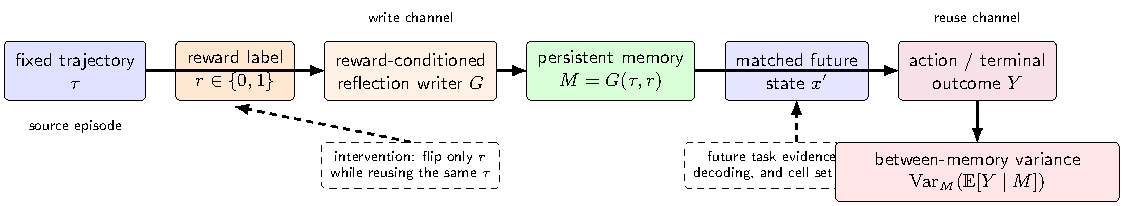
\includegraphics[width=\linewidth]{figures/fig1_reward_write_channel.pdf}
\caption{The reward-to-memory-to-outcome channel. The source trajectory is fixed while the reward label selects the reflection writer. The resulting persistent memory is then injected into a matched held-out task packet under a fixed policy configuration. Repeated outcomes identify the between-memory component of run variance.}
\label{fig:write}
\end{figure}

For a matched future task state $x'$, let $Y$ denote a downstream behavioral or terminal outcome under retrieved memory $M$. The reuse-stage contrast is
\begin{equation}
\Delta_Y(x')=
\mathbb{E}[Y\mid do(M=M(0)),x']-
\mathbb{E}[Y\mid do(M=M(1)),x'].
\label{eq:terminal-contrast}
\end{equation}
The future task evidence and policy configuration are held fixed across the pair. This separates variation introduced by persistent memory state from variation in the observed future state.

\subsection{Variance amplification}
Across self-improvement runs, reward errors can cause different memories to be written from otherwise comparable experiences. Let $M$ denote the persistent memory state available to later tasks. The law of total variance gives
\begin{equation}
\mathrm{Var}(Y)=
\mathbb{E}_{M}[\mathrm{Var}(Y\mid M)]
+\mathrm{Var}_{M}(\mathbb{E}[Y\mid M]).
\label{eq:variance}
\end{equation}
The second term is the component induced by variation in persistent memory state. If reward corruption changes which memory is written and the paired memories produce different conditional success probabilities, reward uncertainty contributes directly to this term. Section~\ref{sec:variance} estimates the paired conditional effect and converts it into an explicit corruption-rate variance curve.

This channel is immediate for external-memory agents. No parameter update is required: a mislabeled episode can change the context available to the very next retrieval.
